\section{内存管理}
\subsection{内存基本管理}

\subsubsection{基本原理和要求}
内存管理的主要功能有:
\begin{enumerate}
    \item 内存空间的分配与回收
    \item 地址转换
    \item 内存空间的扩充
    \item 内存共享
    \item 存储保护
\end{enumerate}

\paragraph{程序的链接与装入}需要 编译, 连接, 装入. 

动态装载(dynamic loading): 一个例程以可重定位装载格式(relocatable load format)存储在磁盘上, 被调用时,就动态地被装载到内存中. 

\paragraph{逻辑地址与物理地址}区分物理地址(physical address)和虚拟地址(virtual address),后者也叫逻辑地址(logical address). 

内存管理单元(memory management unit, MMU)实现从虚拟地址到物理地址的映射的硬件. TBL 也属于 MMU 的一部分. 

\paragraph{内存保护}base 和 limit 两个上下限寄存器来实现框定进程的内存空间, 始于 base 寄存器中存储的地址,终于 base + limit 对应的地址. 内存保护也是通过 MMU实现的. 

\subsubsection{Contiguous Memory Allocation(连续内存分配)}

\paragraph{固定划分(fixed partition)}内存空间划分为若干固定大小的区域,每个分区只分配一个进程. 可能导致内部碎片(internal fragmentation), 即分配量大于进程实际需求量. 

\paragraph{可变划分(variable partition)}只要是空闲且足够大的连续内存区域都可以被分配. 长时间运行后导致外部碎片(external fragmentation), 即存在大量较小的,难以利用的 holes. 

可以使用 First Fit, Best Fit, Worst Fit 等分配策略以减少外部碎片. 

\subsubsection{Paging}
进程中的块称为页或页面(Page),内存中的块称为页框或页帧(Page Frame). 外存也以同
样的单位进行划分,直接称为块或盘块(Block). 进程在执行申请内存时,即要为每个Page分配内存中可用Frame,这就产生了Page和Frame的一一对应。

\paragraph{地址结构}前一部分为页号(page number)$p$,后一部分为页内偏移量(page offset)$d$. 对于 page size 为 4KB 的页,page offset 需要有 $\log_2 4096=12$ 位。

\begin{figure}[H]
    \centering
    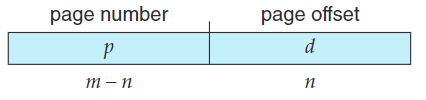
\includegraphics[width=0.618\linewidth]{pic/OS8/address}
    \caption{address}
\end{figure}


\paragraph{页表(page table)}存储逻辑的页到物理的帧的映射关系. 从虚拟地址到物理地址的映射,实际上就是在页表中查询虚拟地址中的 page number,将其换为 frame number,再直接拼接 offset 就行了. 

% \begin{figure}[H]
%     \centering
%     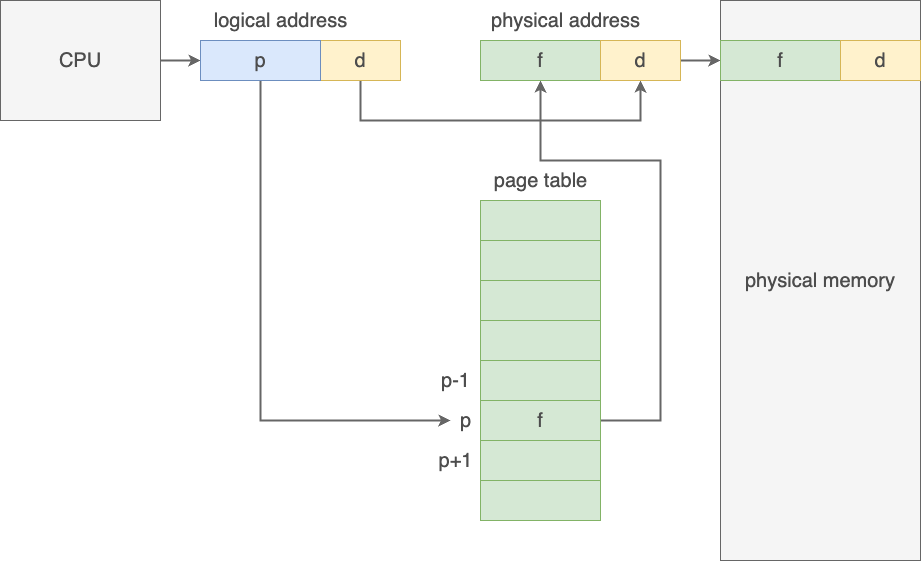
\includegraphics[width=0.618\linewidth]{pic/OS-CheatSheet/page table.png}
%     \caption{地址转化}
% \end{figure}

% \begin{figure}[H]
%     \centering
%     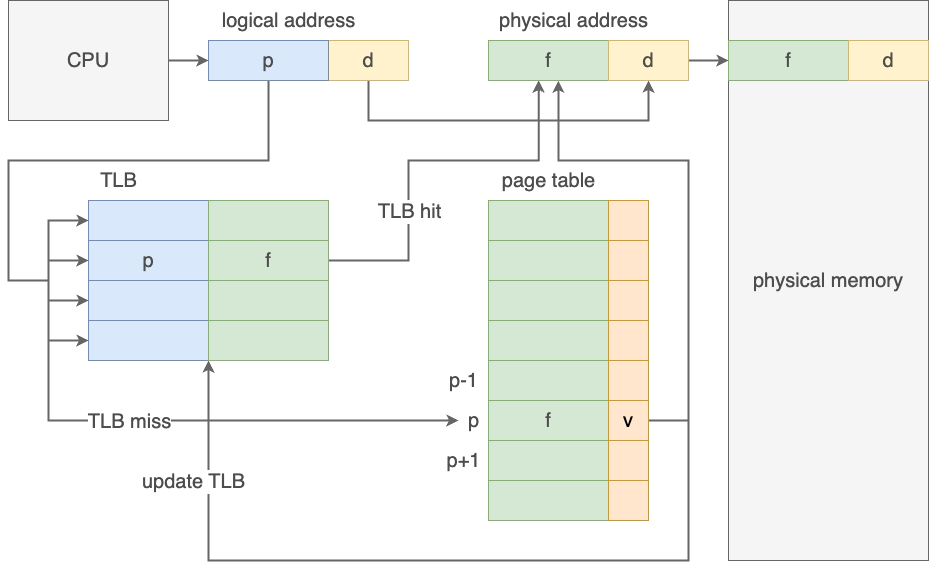
\includegraphics[width=0.618\linewidth]{pic/OS-CheatSheet/地址转换 with tlb}
%     \caption{地址转换 with tlb}
% \end{figure}

\begin{figure}[H]
    \centering
    \begin{minipage}{0.48\linewidth}
        \centering
        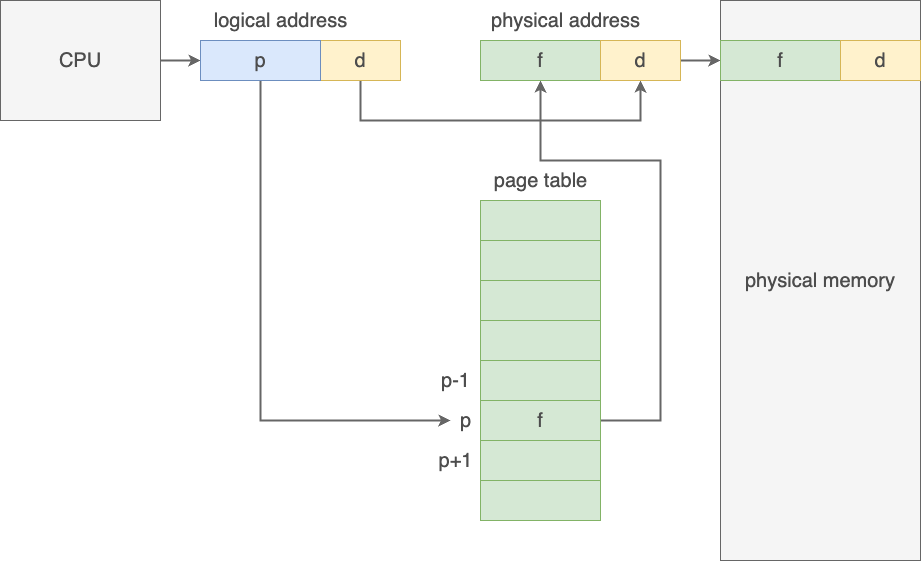
\includegraphics[width=\linewidth]{pic/OS-CheatSheet/page table.png}
        \caption{地址转化}
    \end{minipage}
    \begin{minipage}{0.48\linewidth}
        \centering
    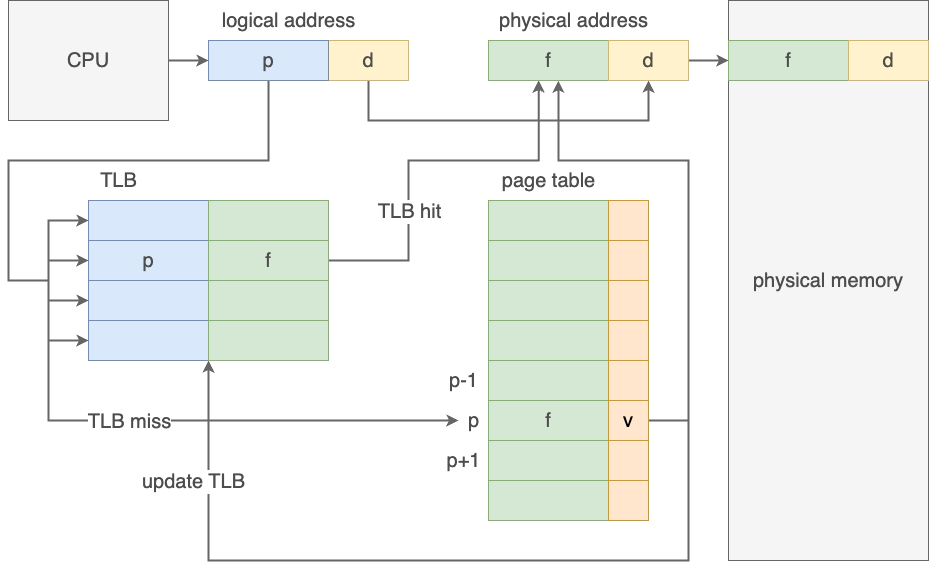
\includegraphics[width=\linewidth]{pic/OS-CheatSheet/地址转换 with tlb}
    \caption{地址转换 with tlb}
    \end{minipage}
    % \caption{}
\end{figure}


\paragraph{硬件支持}页表应当作为一个进程的元信息被维护. 被放在内存中, 页表基址寄存器(page-table base register, PTBR)维护一个指向页表的指针来. 每个进程有一个 PTBR. 

页表缓存(translation look-aside buffer, TLB): 加速页表的维护, 页号和帧号以键值对的形式存储在 TLB 中. 

Associative Lookup $=\epsilon$ time unit. Assume memory cycle time is $t$ ms. Hit ratio $=\alpha$

有效内存访问时间(effective access time, EAT):
\begin{align*}
    EAT &= (t+\epsilon)\alpha+(2t+\epsilon)(1-\alpha)\\
    &=(2-\alpha)t+\epsilon 
\end{align*}


\paragraph{共享页(shared page)}多个页可以对应同一个帧. 提高代码重用率. 

\subsubsection{页表设计改进}
\paragraph{分层分页(hierarchical paging)}典型的就是二级页表(two-level page table). linux 最高可到七级. 

\paragraph{哈希页表(hashed page table)}维护了一张哈希表,以页号的哈希为索引,维护了一个链表,每一个链表项包含页号、帧号、和链表 next 指针,以此来实现页号到帧号的映射.

\paragraph{反式页表(inverted page table)}以物理地址为索引维护映射关系. 使用 content-addressible memory (CAM) 特殊硬件加速. 

\subsubsection{Swapping}
进程可以临时从存储器交换到后备存储器,然后被带回存储器以继续执行。

%TODO \subsubsection{Segmentation}
\subsection{虚拟内存管理}
仅仅一部分在 memory 的程序需要运行. 所以逻辑内存可以大于物理内存. 甚至可以把虚地址扩展到和外存一样大. 

\subsubsection{Demand Paging(请求式调页)}
只把被需要的页载入内存

\paragraph{Valid-Invalid Bit}每个 page table entry (PTE) 会有一个 bit 标识所指页是否 valid. 

\paragraph{Page Fault}当所要访问的页面不在内存中时,便产生一个Page Fault. 
\begin{enumerate}
    \item 对地址, 检查一张 PCB 里的内部表:
    \subitem 若无效引用 $\to$ abort
    \subitem 若只是并没有被分配, 继续
    \item 从可用帧列表里拿出 frame 用来写入
    \subitem 如果可用帧列表为空,则进行页置换
    \item 开始从后备存储读取内容,并写入 frame
    \item 完成读写后,更新内部表和页表等元信息
    \item 重新执行引起 page fault 的 instruction
\end{enumerate}

% \paragraph{A Page Fault Causes The Following}


\paragraph{Performance of Demand Paging}Page Fault Rate: $0\le p \le 1$

\begin{align*}
    EAT =& (1-p)\times \text{memory access}\\
        & + p \left( \begin{array}{rl}
              &\text{page fault overhead}\\
            + &\text{swap page out}\\
            + &\text{swap page in}\\
            + &\text{restart overhead}
        \end{array} \right)
\end{align*}
\subsubsection{Copy-on-Write}
fork 后, 只有当子进程需要发生内容修改的时候,才真正去复制父进程的内容

\subsubsection{Allocation of Frames}
维护可用帧列表(free-frame list),在 demand paging 系统里记录当前哪些帧是空闲的。

对于单个process 分配的 frames数量,存在一个较严格的分配上下界
\begin{enumerate}
    \item 不能大于 free-frame 总量
    \item 不能小于 process ``执行每一条指令所需要涉及的 frames'' 的最大值
\end{enumerate}

早期分配算法(frame-allocation algorithm)主要有这么两种:
\begin{enumerate}
    \item Equal allocation: 每一个进程被分配的 frame 总量都相同
    \item proportional allocation: 按进程的大小来分配
\end{enumerate}

\subsubsection{Page Replacement}
用一个修改位(dirty bit 或 modified bit)来记录页是否被修改过. 

被替换的帧称为牺牲帧(victim frame)

\paragraph{Optimal}选之后再也不会被用到的或下一次用到的时间最晚的页作为 victim frame. 理论上最优. 
\paragraph{FIFO}选择正在使用中的、最早进入内存的 frame 作为 victim frame
\paragraph{LRU}选择最久没被访问过的 frame 作为 victim. 但维护``最久没被访问过''这个信息并不容易, 可以使用计数器或链表序列维护. 
\paragraph{LRU Approx}使用一些方式近似LRU
\begin{enumerate}
    \item Reference-Bits: 在初始化时被置 0;被使用时置 1. 替换 0 的 frame. 
    \item Second-Chance Algorithm: 循环地遍历 frames, 检测 reference bit, 若1则置0, 若0替换. 
    \item Enhanced Second-Chance Algorithm / NRU: 二元组维护 (dirty, reference), 循环地遍历四次 frame, 依次寻找 (0,0), (0,1), (1,0), (1,1)的替换. 
\end{enumerate}

\paragraph{置换范围}replacement 分为 local 和 global
\begin{itemize}
    \item local replacement 只发生在属于当前进程的帧中
    \item global replacement 的 scope 是所有帧
\end{itemize}

\subsubsection{Thrashing(颠簸)}
频繁的 paging 活动, 几乎所有 frames 都正在被使用. 

\paragraph{Priority}用 priority replacement algorithm 来解决

\paragraph{Working Set}指在某段时间间隔内,进程要访问的页面集合。工作集$W$可由时间$t$和工作集窗口大小$\Delta$来确定。工作集反映了进程在接下来的一段时间内很有可能会频繁访问的页面集合, 若working set 的大小之和大于可用 frame 的数量, 就会出现 thrashing. 

\subsubsection{内存映射文件(Memory-Mapped Files)}
将磁盘文件的全部或部分内容与进程虚拟地址空间的某个区域建立映射关系,便可以直接访问被映射的文件,而不必执行文件I/O操作,也无须对文件内容进行缓存处理。

\subsubsection{Allocating Kernel Memory}
Often allocated from a free-memory pool

\paragraph{Buddy 系统}用来分配物理连续的内存,它由 power-of-2 allocator 实现

当 kernel 需要 $n$ KB 的内存时候,Buddy system 会分配一块 $2^{\lceil \log_2 n \rceil}$ KB 的空间. 

其也可以通过 coalesce 相邻的空闲块来形成更大的内存块. 

\paragraph{Slab 分配}预先了解到 kernel 内的常见数据结构(被称为各种 object)的大小,并预先准备好对应粒度的小内存块,注册到每类 object 的 cache 里. 当一个 object 需要使用内存时,就查询对应的 cache 里是否有空闲的内存块,如果有就分配给它,如果没有就向 Buddy system 申请. 